\section{Players}

The Player class can be seen at figure \ref{fig:Player class}. One of the more special aspects of the Player class is the two kinds of figure it holds. One for when he is selected and one for when he is not. A comparison of the two can be seen at figure \ref{fig:PlayerFigure}.\\

\begin{figure}
	\centering
	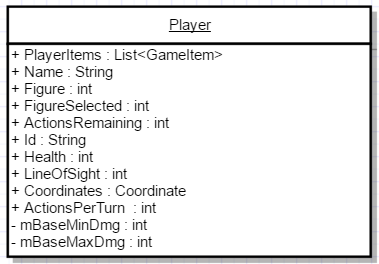
\includegraphics[width=0.8\textwidth]{images/ClassPlayer.png}
	\caption{Player class}
	\label{fig:Player class}
\end{figure}

Another thing that is unique for the player class is the PlayerItems that is a list of GameItems. These items is used to boost the player stats when the player is fighting monsters. The damage a player can give is split into two different properties max and min. The last unique state for the player is the LineOfSight which describes how many tiles a player can see. 

\begin{figure}
		\centering
	\begin{minipage}{0.48\textwidth}
		
\includegraphics{images/player_old_man.png}
		\raggedleft
	\end{minipage}
	\begin{minipage}{0.48\textwidth}
		
\includegraphics{images/player_old_man_selected.png}
	\end{minipage}
		\caption{Player figure comparison}
	\label{fig:PlayerFigure}
\end{figure}

